\documentclass{article}
\usepackage{multirow}
\usepackage{hyperref}
\usepackage{algorithm2e}
\usepackage{graphicx}
\usepackage{amsmath}
\usepackage{amssymb}
\hypersetup{
    colorlinks=true,
    linkcolor=magenta,
    urlcolor=blue
    }
\urlstyle{same}
% \graphicspath{ {./images/} }
\RestyleAlgo{ruled}
\SetKwComment{Comment}{/* }{ */}


\title{Homework Set 3: Monte Carlo Simulations and Numerical Methods for ODEs}
\author{
AMS 326-1: Numerical Analysis, Spring 2025 \\
Joe Martinez
}
\date{April 22, 2025}



\begin{document}
\maketitle

% TODO: Make introductions, descripe the language used, the libraries, and where the code lives on Github
All calculations for this assignement are done in Python, with the source code submitted with this report as hw3.py. The Python libraries used for this project are Shapely, SciPy, Numpy, matplotlib, sys, random, and math. For problems that take more than a second, a progress bar is shown in the terminal when the script is running.

\section{Buffon's Varying Sized Disks (Problem 3-1)}

% Description
Similar to the Buffon's Needle problem, we were tasked to find the probability a randomly thrown disk crossing at least 1, 2, 3, or 4 lines with disks of different diameters for each scenario. Our approach to the solution was to simulate each scenario using 4,444,444 disks over 1000 lines. The different sizes for disk diameter were:

\[ d = \frac{1}{10} \text{,} \frac{2}{10} \text{,} \frac{3}{10} \text{,} \frac{4}{10} \text{,} \frac{5}{10} \text{,} \frac{6}{10} \text{,} \frac{7}{10} \text{,} \frac{8}{10} \text{,} \frac{9}{10} \text{,} \frac{10}{10} \text{,} \frac{15}{10} \text{,} \frac{20}{10} \text{,}  \frac{30}{10} \]

% Explanation of Algorithm
Simulating our disks and lines, the lines lied on the vertical axis with a distance of 1 between consecutive lines, and we  randomly sampled a horizontal x-axis value from a uniform distribution for the center of each disk. Since the lines are in the vertical axis, there was no need to randomly sample y values for each disk since it doesn't affect determining if the disk crossed a line.

Determining whether a disk crossed a line was done by iterating through the ith closets pair of lines to the left or right of the disk and calculating the distance between the center of disk to each line. For example, for the first iteration, d1 would be the distance to the 1st closest line to the left of the disk, and d2 would be to the 1st closest line to the right of the disk. The disk crosses a line if the distance to that line is smaller than or equal to the radius of the disk. We iterate through the pairs of lines until we find that both distances are larger than the radius of the disk, counting each crossed line each iteration.

Since our goal was to calculate the percentage of  disks that cross as least 1,2,3 and 4 lines, the probability that a disk crossed at least n lines is

\[
    P(lines =n)=\frac{\sum_{i=n}^l\text{\# of disks that crossed i lines}}{\text{total \# of disks}}
\]

where $l$ is the total number of possible lines that a disk can cross, which is $\lfloor{d / 1}\rfloor + 1$. The pseudocode for this algorithm is seen in Algorithm \ref{alg:disk}. 



% Algorithm for classifying random disks
\begin{algorithm}[hbt!]
    \caption{Buffon Disk Monte Carlo Simulation}\label{alg:disk}
    \KwIn{The number of disks to throw $disks$, the diameter of each disk $disk_d$, the number of needles $needles$, and the seperation between needles $lineWidth$}
    \KwOut{A array of intergers descriping how many disks landed on i lines, where i is the ith index of the array}
    \SetKwProg{BuffonDisks}{BuffonDisks}{}{}
    \SetKw{KwBy}{by}
\BuffonDisks{$(disks, disk\_d, needles, lineWidth)$}{
    $disk\_r \gets disk\_d / 2$\;
    $maxLines \gets \lfloor{disk\_d / lineWidth + 1}\rfloor$\;
    $diskTouchLines \gets$ Initialize a new array of size $maxLines + 1$\;
    
    \For{$i \gets$ 0 $\KwTo$ $disks$}{
        $lines \gets 0$\;
        $step \gets 0$\;
        $d1 \gets 0$\;
        $d2 \gets 0$\;
        \While{$d1 < disk\_r$ or $d2 < disk\_r$}{
            $x \gets $\text{sample from} $Uniform(0, maxLines)$\;
            $prevLine \gets \lfloor{x - step}\rfloor$\;
            $nextLine \gets \lfloor{x + step}\rfloor$\;
            $d1 \gets x - prevLine$\;
            $d2 \gets nextLine - x$\;

            \eIf{$d1 == 0$ or $d2 == 0$}
            {
                $lines \gets lines + 1$\;
            }{
                \If{$d1 < disk\_r$ and $prevLine \geq 0$}
                {
                    $lines \gets lines + 1$\;
                }
                \If{$d2 < disk\_r$ and $nextLine \leq lastLine$}{
                    $lines \gets lines + 1$\;
                }
            }
            $step \gets step + 1$
        }
    }
    \For{$i \gets 1$ \KwTo $1$ \KwBy $-1$}{
        $disksTouchLines[i-1] \gets disksTouchLines[i-1] + disksTouchLines[i]$\;
    }
}
\end{algorithm}

% Table of results for the different disks
Running Algorithm \ref{alg:disk} for our list of varying disk diameters, the probabilities can be seen in Table \ref{tbl:disk}. An important note is that for a disk diameter of 1, the possibility of crossing 2 lines is incredible small, but not impossible. Same logic applies for a disk diameter of 2 with crossing 3 lines and for the a disk diamtere of 3 with crossing 4 lines. The probability distribution function (PDF) of a disk crossing 0, 1, 2, 3, and 4 lines based on disk diameters are in Figures \ref{fig:l0}, \ref{fig:l1}, \ref{fig:l2},\ref{fig:l3}, and \ref{fig:l4} respectively. 

\begin{table}
    \centering

    \begin{tabular}{|c||c|c|c|c|c|}
        \hline
        \multirow{2}{*}{Disk Diameter} & \multicolumn{5}{|c|}{Lines Crossed} \\
        \cline{2-6} & 0 & 1 & 2 & 3 & 4 \\
        \hline
        0.1 & 0.899968 & 0.100032 & 0.0 & 0.0 & 0.0 \\
        0.2 & 0.799593 & 0.200407 & 0.0 & 0.0 & 0.0 \\
        0.3 & 0.699829 & 0.300172 & 0.0 & 0.0 & 0.0 \\
        0.4 & 0.600033 & 0.399967 & 0.0 & 0.0 & 0.0 \\
        0.5 & 0.499997 & 0.500003 & 0.0 & 0.0 & 0.0 \\
        0.6 & 0.400116 & 0.599884 & 0.0 & 0.0 & 0.0 \\
        0.7 & 0.300230 & 0.699770 & 0.0 & 0.0 & 0.0 \\
        0.8 & 0.199904 & 0.800096 & 0.0 & 0.0 & 0.0 \\
        0.9 & 0.099597 & 0.900403 & 0.0 & 0.0 & 0.0 \\
        1.0 & 0.0 & 1.0 & 0.0 & 0.0 & 0.0 \\
        1.5 & 0.0 & 1.0 & 0.500103 & 0.0 & 0.0 \\
        2.0 & 0.0 & 1.0 & 1.0 & 0.0 & 0.0 \\
        3.0 & 0.0 & 1.0 & 1.0 & 0.999003 & 0.0 \\
        \hline

    \end{tabular}
    \caption{Probabilities of disks crossing specified lines}\label{tbl:disk}
\end{table}

% Plots for the different lines 
\begin{figure}[hbt!]
    \centering
    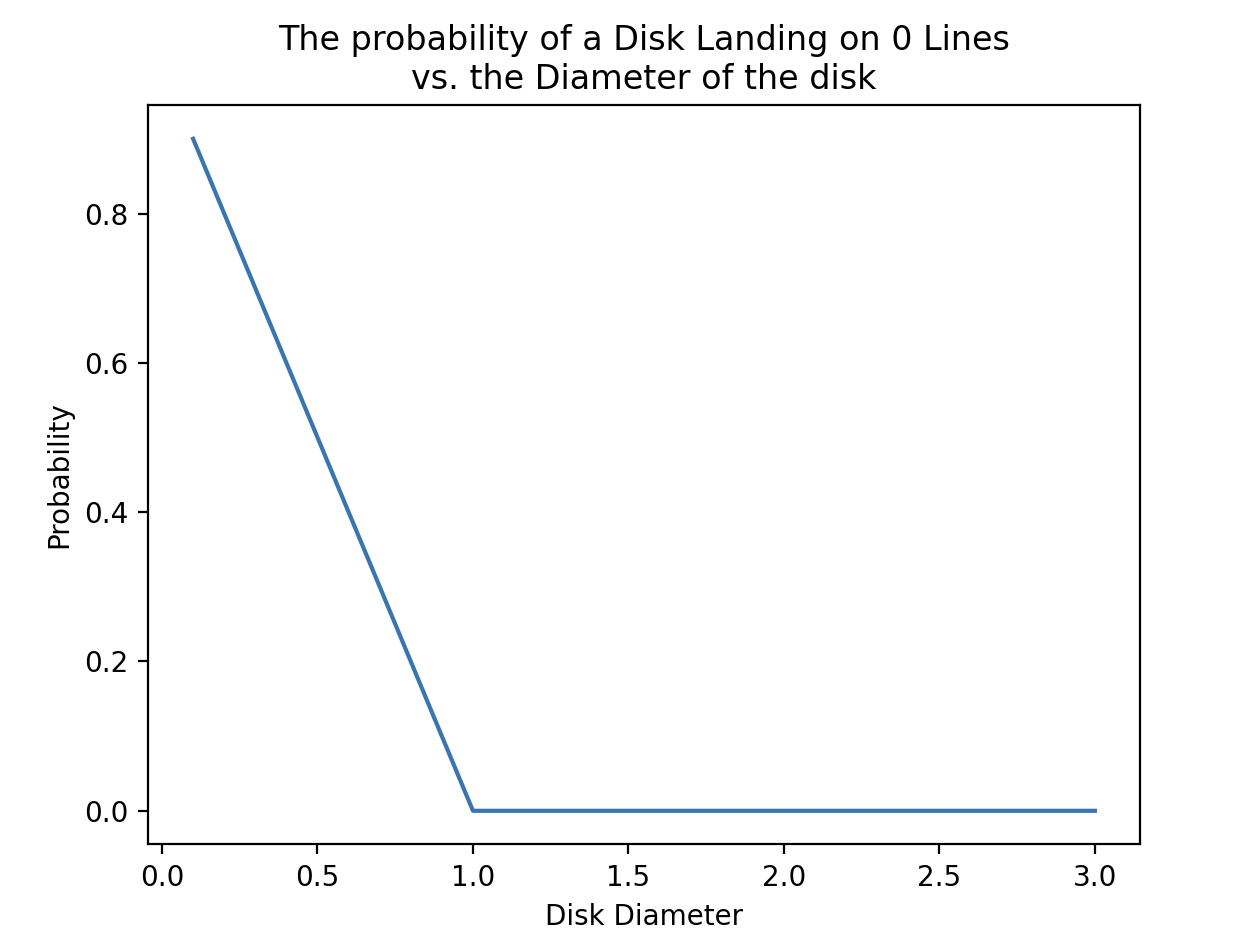
\includegraphics[width=0.95\linewidth]{images/l0.png}
    \caption{PDF of crossing 0 lines based on disk diameter}
    \label{fig:l0}
\end{figure}
\begin{figure}[hbt!]
    \centering
    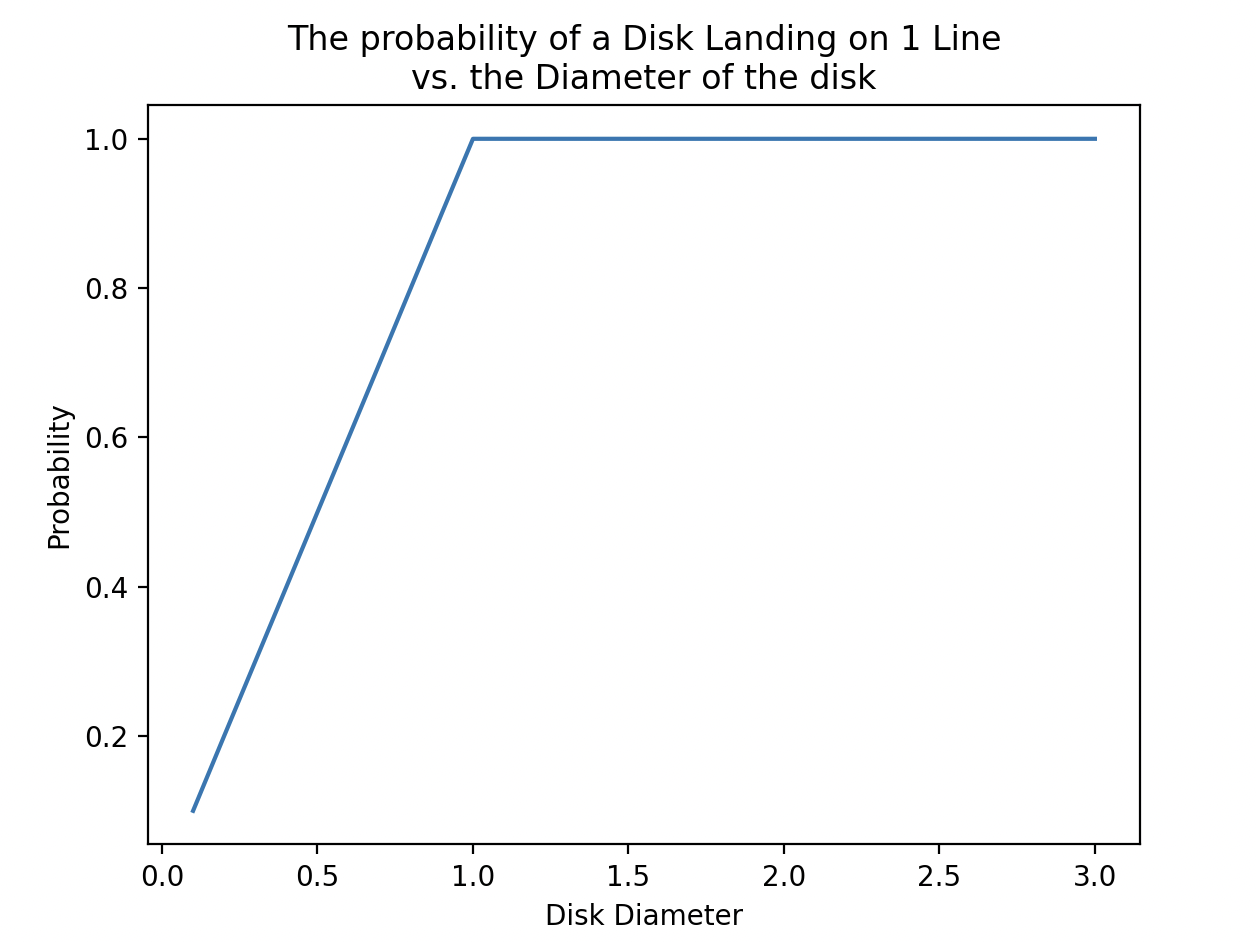
\includegraphics[width=0.95\linewidth]{images/l1.png}
    \caption{PDF of crossing 1 lines based on disk diameter}
    \label{fig:l1}
\end{figure}
\begin{figure}[hbt!]
    \centering
    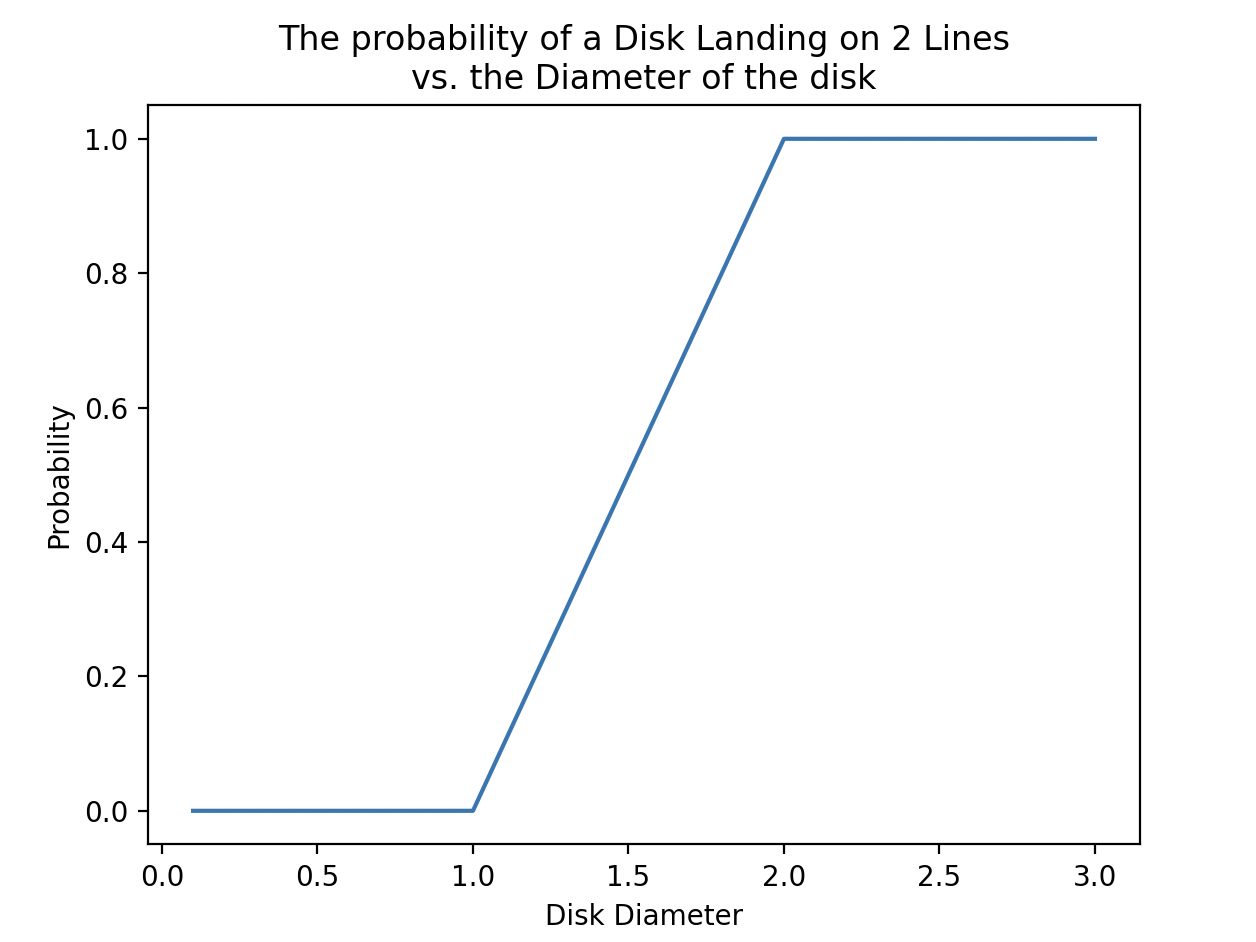
\includegraphics[width=0.95\linewidth]{images/l2.png}
    \caption{PDF of crossing 2 lines based on disk diameter}
    \label{fig:l2}
\end{figure}
\begin{figure}[hbt!]
    \centering
    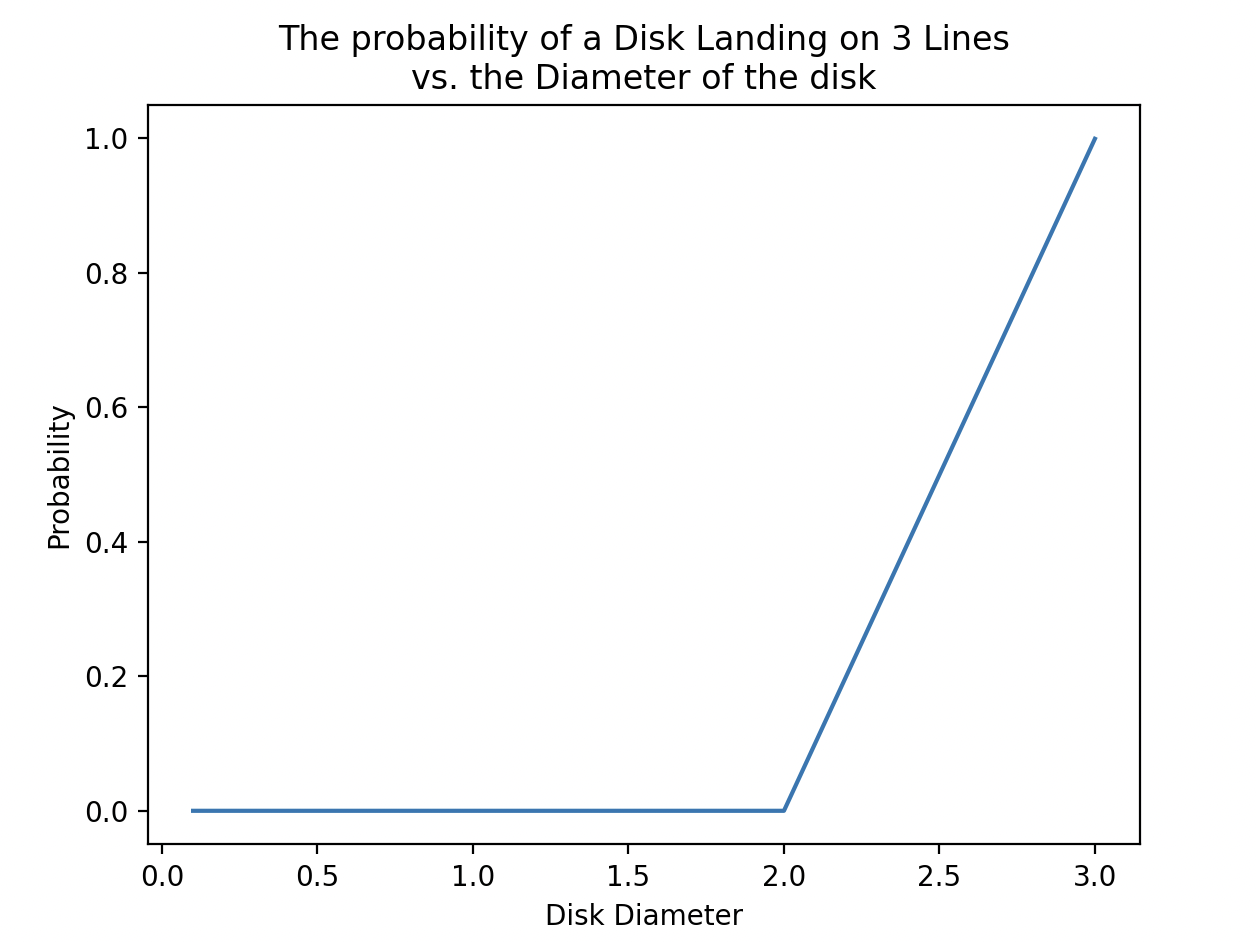
\includegraphics[width=0.95\linewidth]{images/l3.png}
    \caption{PDF of crossing 3 lines based on disk diameter}
    \label{fig:l3}
\end{figure}
\begin{figure}[hbt!]
    \centering
    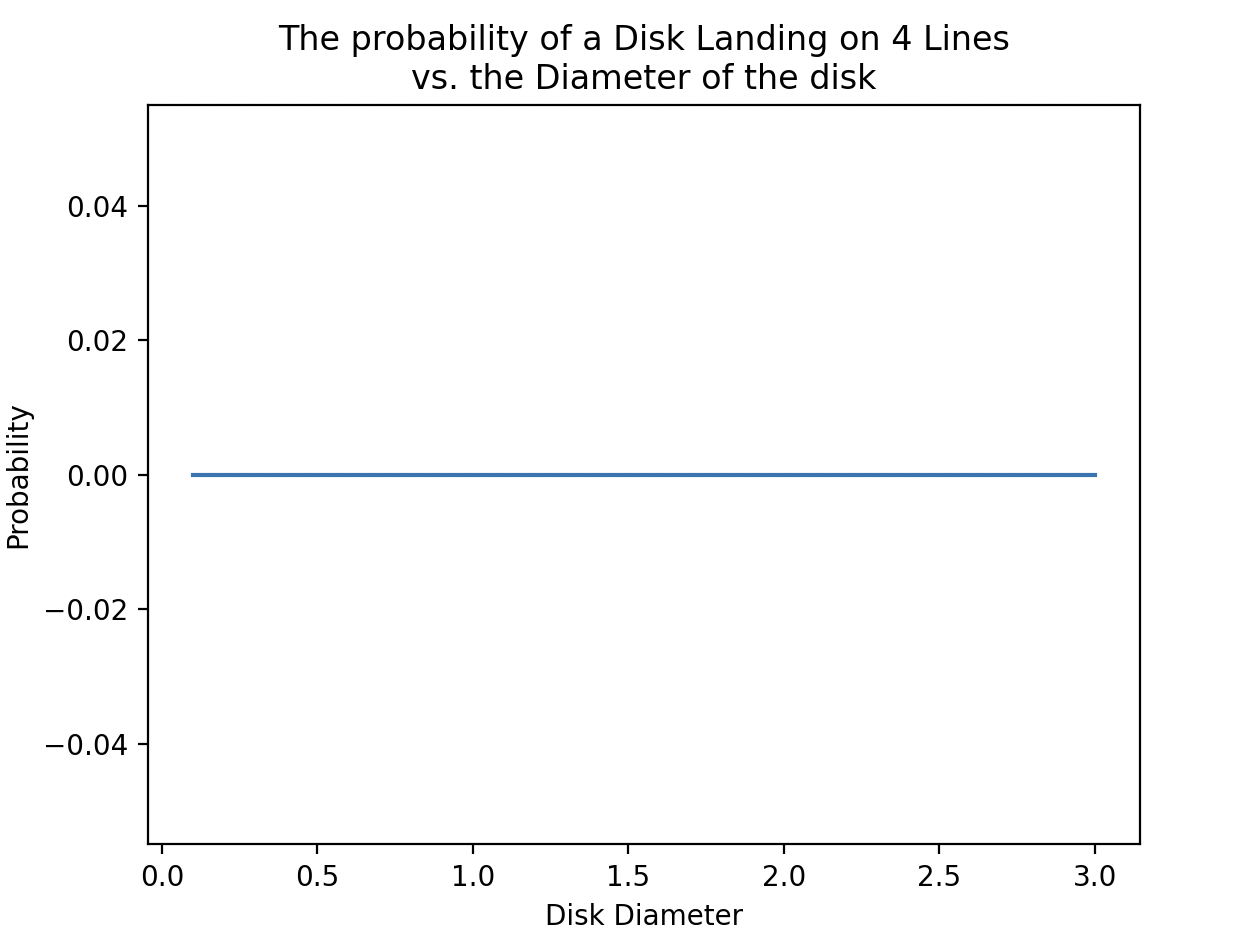
\includegraphics[width=0.95\linewidth]{images/l4.png}
    \caption{PDF of crossing 4 lines based on disk diameter}
    \label{fig:l4}
\end{figure}




\section{Maximum Cut for a 4-leaf Rose Curve (Problem 3-2)}
% Description
Given the 4-leaf "rose" graph $r=sin2\theta$, or $(x^2+y^2)^3=4x^2y^2$ in Cartesian coordinates, our goal was to find the best spot to place a retangular cutter of size $1 \times \frac{1}{\sqrt{2}}$ to maximize the area of the cut. 

% Explanation of algorithm
Our approach to find a maximum area cut from a generally random starting spot was to use the L-BFGS-B algorithm, which is a limited memory numerical optimization algorithm. The BFGS-B algorithm is a quasi-Newton method that approximates the Hessian matrix to perform gradiant desent, finding the local minimum of a function and optimizing it. In this case, the function we want to optimize is the area of the cut applied on the rose graph, aiming for the maximum area. Therefore, as shown in Algorithm \ref{alg:rose}, the aim was to minimize the negative area of the cut area, hence producing a maximum area. The L-BFGS-B algorithm in this case is optimizing Algorithm \ref{alg:area}, the calculation of the area cut from the rose graph and a defined cutter.

% Algorithm for maximizing the area of the cutter
\begin{algorithm}
    \caption{Negative Cutter Area from Rose Curve}\label{alg:area}
    \KwIn{The x, y, and angle of cutter $x$, $y$, and $angle$ respectfully, the rose curve Polygon, $rose$, and a cutter Polygon creating function, $\textbf{createCutter}$.}
    \KwOut{The negative area of the curve}
    \SetKwProg{NegativeIntersectionArea}{NegativeIntersectionArea}{}{}
\NegativeIntersectionArea{$(x, y, angle, rose, \textbf{createCutter})$}{
    $cutter \gets \textbf{createCutter}(x,y, angle)$\;
    $intersection \gets$ the intersection of $rose$ and $cutter$\;
    \Return the negative of the intersection area
}
\end{algorithm}


\begin{algorithm}
    \caption{Maximum Area Cut For Rose Curve Monte Carlo}\label{alg:rose}
    \KwIn{A polygon representing the rose curve to maximize the cut for, $rose$.}
    \KwOut{The maximum area of a cut from curve, and both the location fo the cutter and a plot of the cutter are outputted}
    \SetKwProg{MaxRoseCut}{MaxRoseCut}{}{}
    \SetKw{KwOutput}{output}
\MaxRoseCut{(rose)}{
    % $rose \gets$ a Polynomial representation of the Rose graph\;
    $init\_x \gets$ sampled from $Uniform(-0.25, 0.25)$\;
    $init\_y \gets$ sampled from $Uniform(-0.25, 0.25)$\;
    $init\_theta \gets$ sampled from $Uniform(0, 2\pi)$\;
    $init\_params \gets [init\_x, init\_y, init\_theta]$\;
    $bounds \gets [(-0.25, 0.25), (-0.25, 0.25), (0, 2\pi)]$\;
    $results \gets \textbf{L-BFGS-B}(\textbf{NegativeIntersectionArea}, init\_params, bounds, rose)$\;
    \KwOutput graph of best cutter from results\;
    \Return max area from results\;
}
\end{algorithm}


% Results (two options)
Using Algorithm \ref{alg:rose} on two different occasions, starting from a random spot in the range $-0.25 \leq x \leq 0.25$ and $-0.25 \leq y \leq 0.25$ (using the heatmap for maximum area), two maximum area cuts were found. Figure \ref{fig:rose1} shows a maximum cut of area 0.5878186487084814, placing the cutter at $x= 2.557233\times 10^{-6}$, $y=-2.768929\times 10^{-5}$, and an angle of $3.141593297595777 \approx 2\pi=0^o$. Figure \ref{fig:rose2} shows a maximum cut of area 0.5878186629229423, placing the cutter at $x= 1.403466\times 10^{-9}$, $y=-7.215794\times 10^{-6}$, and an angle of $4.712389002212077 \approx 2\pi + \frac{\pi}{2} = 90^o$.
% Plots
\begin{figure}[hbt!]
    \centering
    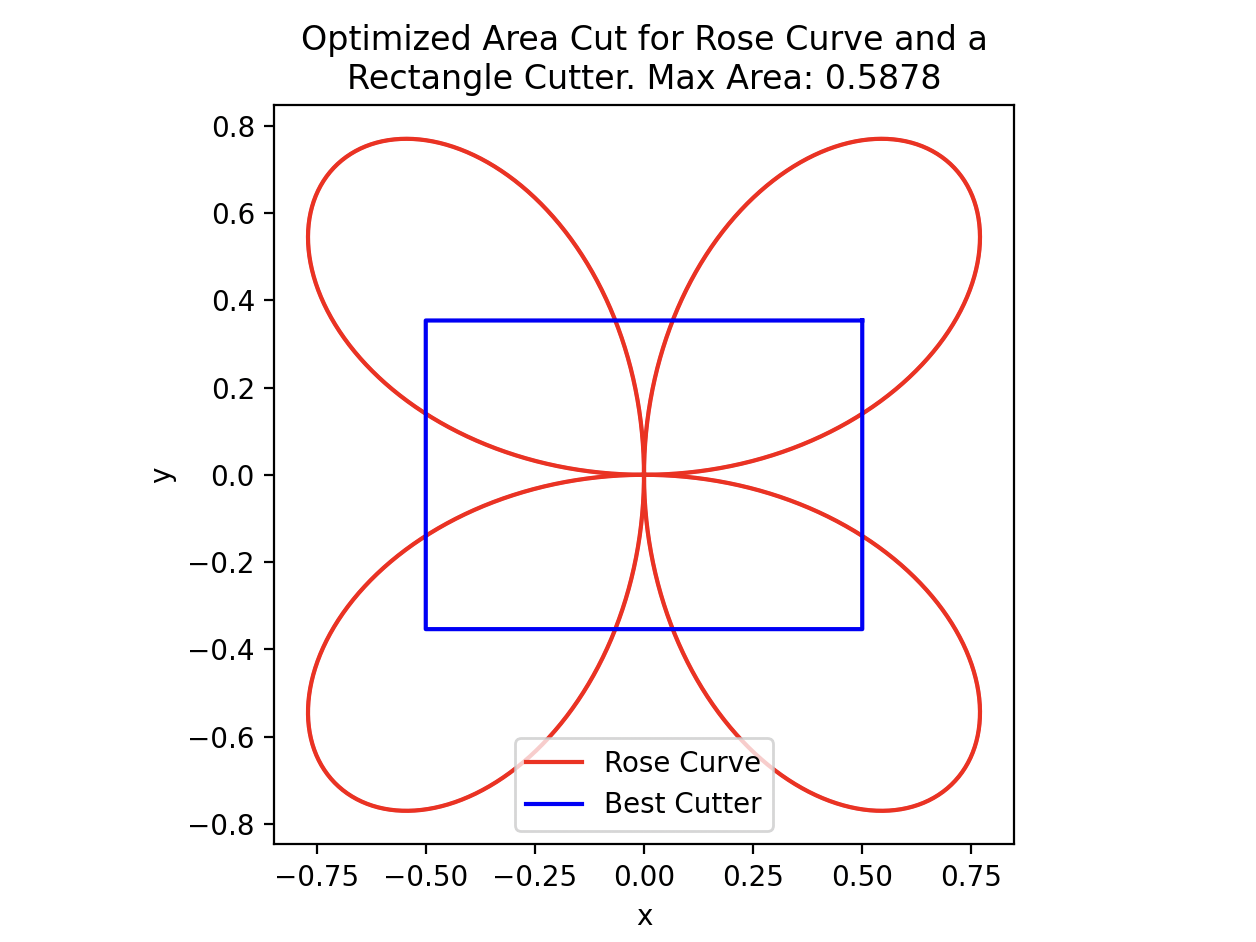
\includegraphics[width=0.95\linewidth]{images/rose1.png}
    \caption{Maximum area cut with an angle of 0 degrees}
    \label{fig:rose1}
\end{figure}
\begin{figure}[hbt!]
    \centering
    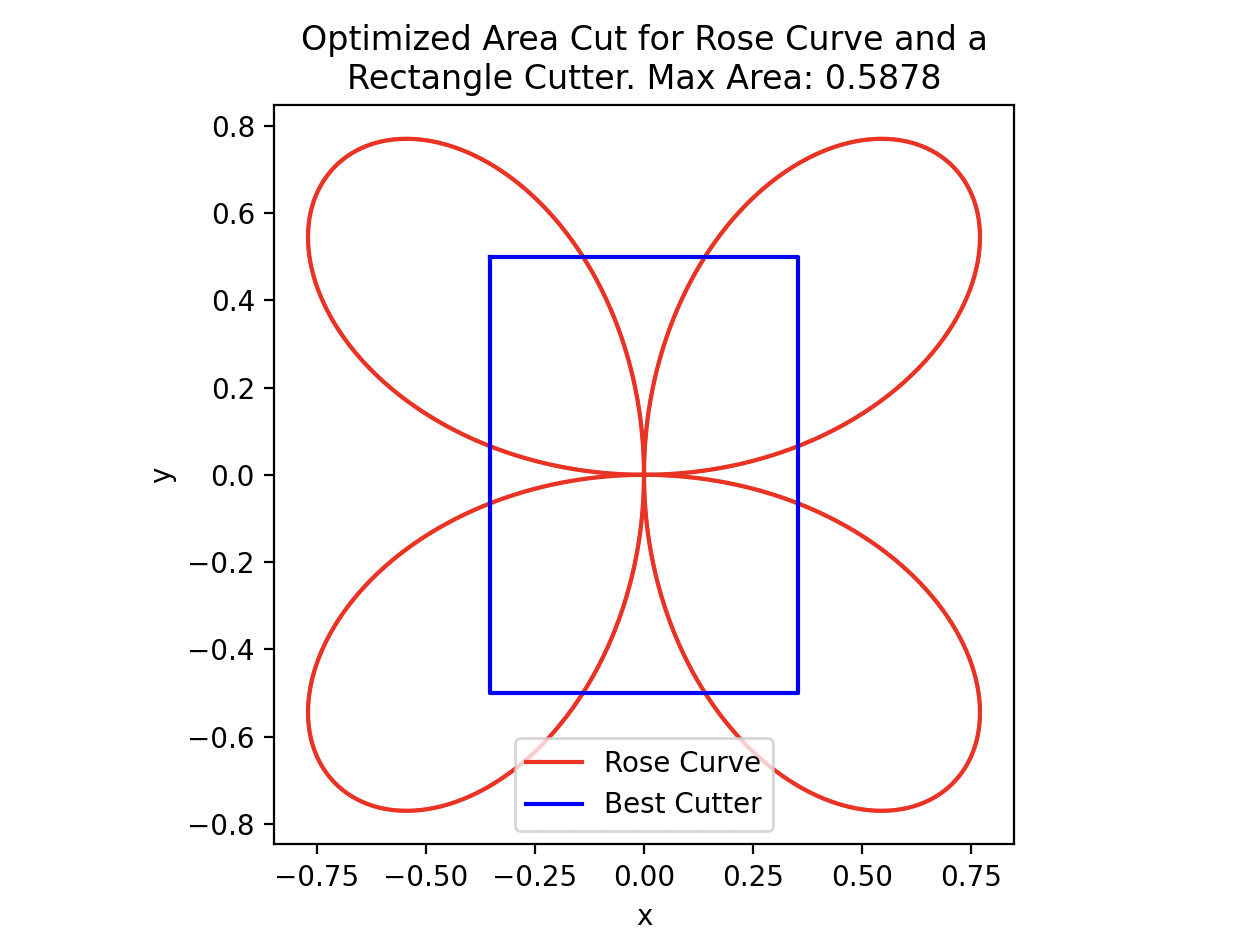
\includegraphics[width=0.95\linewidth]{images/rose2.png}
    \caption{Maximum area cut with an angle of 90 degrees}
    \label{fig:rose2}
\end{figure}


\section{The Trajectory of a Plane (Problem 3-3)}
% Description
A plane is flying starting from ($a$, 0) to an airport at (0,0) with a constant speed of $v_0$ always heading towards the airport, and a constain wind of speed of $w$ in the positive y direction. Both of these fact combined create an ordinary differential equation detailing the change in y position with respect to the change in x position of the plane:
\[
\frac{dy}{dx} = \frac{y}{x}-k\sqrt{1+(\frac{y}{x})^2}
\]
where $k=\frac{w}{v_0}$. Given the initial values of $a=100$, $w=44$, and $v_0=88$, our goal is to map out the plane's trajectory using this ordinary differential equation.

% ODE equation
% Runge-Kutta Method Explanation
The Runge-Kutta 3 (RK3) method uses slopes of two predicted future point to calculate an averaged weighted slope to numerically estimate a point at a $h$ independent variable distance away from the starting independent variable point. This method can be used iteratively, plugging in new points into the method to estimate even furthur points from the stating point. 

% Algorithm for trajectrory simulation
\begin{algorithm}
    \caption{Runge-Kutta 3 Method for Plane Trajectory}\label{alg:plane}
    \KwIn{The starting x and y coordinates of the plane, $x$ and $y$, the differential equation defined as dy/dx, $f(x,y)$, and the incremental step $h$}
    \KwOut{A list of values x and y values indicating the airplane's trajectory, as well as a plot of the trajectory}
    \SetKw{KwOutput}{output}
    \SetKwProg{SimulatePlane}{SimulatePlane}{}{}
\SimulatePlane{$(startX, startY, h)$}{
    $x \gets startX$\;
    $y \gets startY$\;
    $trajectory \gets$ initialize new array\; 
    \While{$x \geq 0$ and $y \geq 0$}{
        $k_1 \gets f(x,y)$\;
        $k_2 \gets f(x + \frac{h}{2}, y + \frac{h}{2}k_1)$\;
        $k_3 \gets f(x + h, y - hk_1 + 2hk_2)$\;
        $y \gets y + \frac{h}{6}(k_1 + 4k_2 + k_3)$\;
        $x \gets x + h$

        \If{$x \geq 0$ and $y \geq 0$}{
            append to $trajectory$ $(x, y)$\;
        }
    }
    \KwOutput Plot of $trajectory$\;
    \Return $trajectory$\;
}
\end{algorithm}


% Resulting Trajectory
Inputting our intial values and start from the point (100, 0), and using an $h$ value of $-10^{-4}$, we found the trajectory of the plane to be as shown in Figure \ref{fig:plane}.


\begin{figure}[hbt!]
    \centering
    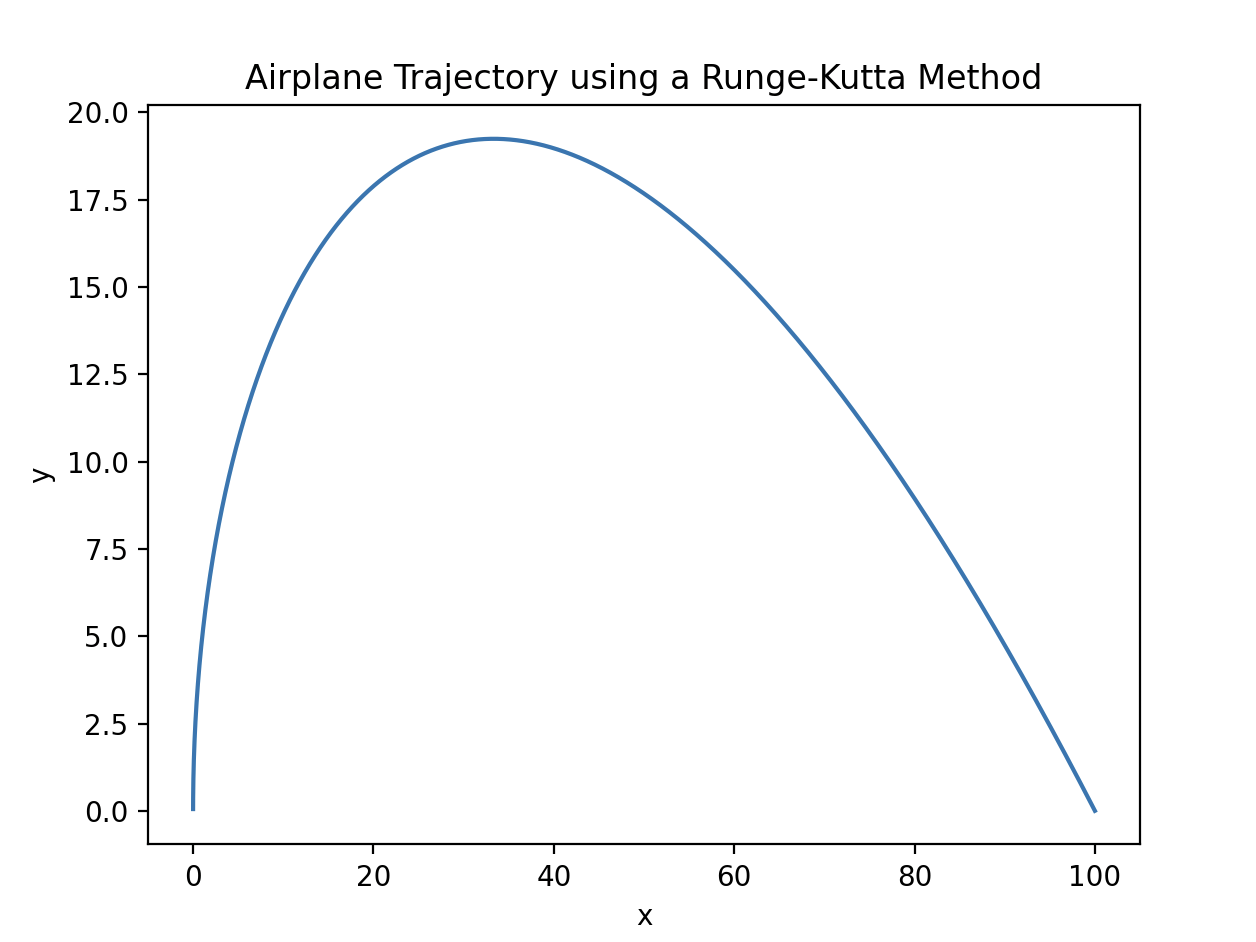
\includegraphics[width=0.95\linewidth]{images/plane.png}
    \caption{The trajectory of the plan estimated with the Runge-Kutta 3 Method, starting at point (100, 0)}
    \label{fig:plane}
\end{figure}



\end{document}